%% uncomment to list all files in log
%\listfiles

\documentclass[12pt]{report}


\usepackage{fontspec}

%\setmainfont[Scale=MatchLowercase]{Lucida Bright}
%\setmonofont{FreeMono}
%\setmonofont{Source Code Pro}
\setmonofont[Scale=MatchLowercase]{Ubuntu Mono}

\usepackage[headings]{fullpage}

% national use characters 
%\usepackage{inputenc}

% ams mathematical symbols
\usepackage{amsmath,amssymb}

% added to support pandoc highlighting
\usepackage{microtype}

\usepackage{makeidx}

% add index and bibliographies to table of contents
\usepackage[nottoc]{tocbibind}

% postscript courier and times in place of cm fonts
%\usepackage{courier}
%\usepackage{times}

% extended coloring
\usepackage{color}
\usepackage[table,dvipsnames]{xcolor}
\usepackage{colortbl}

% advanced date formating
\usepackage{datetime}

%support pandoc code highlighting
\usepackage{fancyvrb}
\DefineShortVerb[commandchars=\\\{\}]{\|}
\DefineVerbatimEnvironment{Highlighting}{Verbatim}{commandchars=\\\{\}}
% Add ',fontsize=\small' for more characters per line

%tango style colors
% \usepackage{framed}
% \definecolor{shadecolor}{RGB}{255,255,255}
% \newenvironment{Shaded}{\begin{snugshade}}{\end{snugshade}}
% \newcommand{\KeywordTok}[1]{\textcolor[rgb]{0.13,0.29,0.53}{\textbf{{#1}}}}
% \newcommand{\DataTypeTok}[1]{\textcolor[rgb]{0.13,0.29,0.53}{{#1}}}
% \newcommand{\DecValTok}[1]{\textcolor[rgb]{0.00,0.00,0.81}{{#1}}}
% \newcommand{\BaseNTok}[1]{\textcolor[rgb]{0.00,0.00,0.81}{{#1}}}
% \newcommand{\FloatTok}[1]{\textcolor[rgb]{0.00,0.00,0.81}{{#1}}}
% \newcommand{\CharTok}[1]{\textcolor[rgb]{0.31,0.60,0.02}{{#1}}}
% \newcommand{\StringTok}[1]{\textcolor[rgb]{0.31,0.60,0.02}{{#1}}}
% \newcommand{\CommentTok}[1]{\textcolor[rgb]{0.56,0.35,0.01}{\textit{{#1}}}}
% \newcommand{\OtherTok}[1]{\textcolor[rgb]{0.56,0.35,0.01}{{#1}}}
% \newcommand{\AlertTok}[1]{\textcolor[rgb]{0.94,0.16,0.16}{{#1}}}
% \newcommand{\FunctionTok}[1]{\textcolor[rgb]{0.00,0.00,0.00}{{#1}}}
% \newcommand{\RegionMarkerTok}[1]{{#1}}
% \newcommand{\ErrorTok}[1]{\textbf{{#1}}}
% \newcommand{\NormalTok}[1]{{#1}}

%espresso style colors
% \usepackage{framed}
% \definecolor{shadecolor}{RGB}{42,33,28}
% \newenvironment{Shaded}{\begin{snugshade}}{\end{snugshade}}
% \newcommand{\KeywordTok}[1]{\textcolor[rgb]{0.26,0.66,0.93}{\textbf{{#1}}}}
% \newcommand{\DataTypeTok}[1]{\textcolor[rgb]{0.74,0.68,0.62}{\underline{{#1}}}}
% \newcommand{\DecValTok}[1]{\textcolor[rgb]{0.27,0.67,0.26}{{#1}}}
% \newcommand{\BaseNTok}[1]{\textcolor[rgb]{0.27,0.67,0.26}{{#1}}}
% \newcommand{\FloatTok}[1]{\textcolor[rgb]{0.27,0.67,0.26}{{#1}}}
% \newcommand{\CharTok}[1]{\textcolor[rgb]{0.02,0.61,0.04}{{#1}}}
% \newcommand{\StringTok}[1]{\textcolor[rgb]{0.02,0.61,0.04}{{#1}}}
% \newcommand{\CommentTok}[1]{\textcolor[rgb]{0.00,0.40,1.00}{\textit{{#1}}}}
% \newcommand{\OtherTok}[1]{\textcolor[rgb]{0.74,0.68,0.62}{{#1}}}
% \newcommand{\AlertTok}[1]{\textcolor[rgb]{1.00,1.00,0.00}{{#1}}}
% \newcommand{\FunctionTok}[1]{\textcolor[rgb]{1.00,0.58,0.35}{\textbf{{#1}}}}
% \newcommand{\RegionMarkerTok}[1]{\textcolor[rgb]{0.74,0.68,0.62}{{#1}}}
% \newcommand{\ErrorTok}[1]{\textcolor[rgb]{0.74,0.68,0.62}{\textbf{{#1}}}}
% \newcommand{\NormalTok}[1]{\textcolor[rgb]{0.74,0.68,0.62}{{#1}}}

%kete style colors
% \newenvironment{Shaded}{}{}
% \newcommand{\KeywordTok}[1]{\textbf{{#1}}}
% \newcommand{\DataTypeTok}[1]{\textcolor[rgb]{0.50,0.00,0.00}{{#1}}}
% \newcommand{\DecValTok}[1]{\textcolor[rgb]{0.00,0.00,1.00}{{#1}}}
% \newcommand{\BaseNTok}[1]{\textcolor[rgb]{0.00,0.00,1.00}{{#1}}}
% \newcommand{\FloatTok}[1]{\textcolor[rgb]{0.50,0.00,0.50}{{#1}}}
% \newcommand{\CharTok}[1]{\textcolor[rgb]{1.00,0.00,1.00}{{#1}}}
% \newcommand{\StringTok}[1]{\textcolor[rgb]{0.87,0.00,0.00}{{#1}}}
% \newcommand{\CommentTok}[1]{\textcolor[rgb]{0.50,0.50,0.50}{\textit{{#1}}}}
% \newcommand{\OtherTok}[1]{{#1}}
% \newcommand{\AlertTok}[1]{\textcolor[rgb]{0.00,1.00,0.00}{\textbf{{#1}}}}
% \newcommand{\FunctionTok}[1]{\textcolor[rgb]{0.00,0.00,0.50}{{#1}}}
% \newcommand{\RegionMarkerTok}[1]{{#1}}
% \newcommand{\ErrorTok}[1]{\textcolor[rgb]{1.00,0.00,0.00}{\textbf{{#1}}}}
% \newcommand{\NormalTok}[1]{{#1}}
%end pandoc code hacks

% jodliterate colors
\usepackage{color}
\definecolor{shadecolor}{RGB}{248,248,248}
% j control structures 
\definecolor{keywcolor}{rgb}{0.13,0.29,0.53}
% j explicit arguments x y m n u v
\definecolor{datacolor}{rgb}{0.13,0.29,0.53}
% j numbers - all types see j.xml
\definecolor{decvcolor}{rgb}{0.00,0.00,0.81}
\definecolor{basencolor}{rgb}{0.00,0.00,0.81}
\definecolor{floatcolor}{rgb}{0.00,0.00,0.81}
% j local assignments
\definecolor{charcolor}{rgb}{0.31,0.60,0.02}
\definecolor{stringcolor}{rgb}{0.31,0.60,0.02}
\definecolor{commentcolor}{rgb}{0.56,0.35,0.01}
% primitive adverbs and conjunctions
%\definecolor{othercolor}{rgb}{0.56,0.35,0.01}   
\definecolor{othercolor}{RGB}{0,0,255}
% global assignments
\definecolor{alertcolor}{rgb}{0.94,0.16,0.16}
% primitive J verbs and noun names
\definecolor{funccolor}{rgb}{0.00,0.00,0.00}    

\usepackage{framed}
\newenvironment{Shaded}{}{}
\newcommand{\KeywordTok}[1]{\textcolor{keywcolor}{\textbf{{#1}}}}
\newcommand{\DataTypeTok}[1]{\textcolor{datacolor}{{#1}}}
%\newcommand{\DecValTok}[1]{\textcolor{decvcolor}{{#1}}}
\newcommand{\DecValTok}[1]{{#1}} 
\newcommand{\BaseNTok}[1]{\textcolor{basencolor}{{#1}}}
\newcommand{\FloatTok}[1]{\textcolor{floatcolor}{{#1}}}
\newcommand{\CharTok}[1]{\textcolor{charcolor}{\textbf{{#1}}}}
\newcommand{\StringTok}[1]{\textcolor{stringcolor}{{#1}}}
\newcommand{\CommentTok}[1]{\textcolor{commentcolor}{\textit{{#1}}}}
\newcommand{\OtherTok}[1]{\textcolor{othercolor}{{#1}}} 
\newcommand{\AlertTok}[1]{\textcolor{alertcolor}{\textbf{{#1}}}}
%\newcommand{\FunctionTok}[1]{\textcolor{funccolor}{{#1}}}
\newcommand{\FunctionTok}[1]{{#1}}
\newcommand{\RegionMarkerTok}[1]{{#1}}
\newcommand{\ErrorTok}[1]{\textbf{{#1}}}
\newcommand{\NormalTok}[1]{{#1}}

% headers and footers
\usepackage{fancyhdr}
\pagestyle{fancy}

\fancyhead{}
\fancyfoot{}

%\fancyhead[LE,RO]{\slshape \rightmark}
%\fancyhead[LO,RE]{\slshape \leftmark}
\fancyfoot[C]{\thepage}
%\headrulewidth 0.4pt
%\footrulewidth 0 pt

%\addtolength{\headheight}{\baselineskip}

%\lfoot{\emph{Analyze the Data not the Drivel}}
%\rfoot{\emph{\today}}

% subfigure handles figures that contain subfigures
%\usepackage{color,graphicx,subfigure,sidecap}
\usepackage{graphicx,sidecap}
\usepackage{subfigure}
\graphicspath{{./inclusions/}}

% floatflt provides for text wrapping around small figures and tables
\usepackage{floatflt}

% tweak caption formats 
\usepackage{caption} 
\usepackage{sidecap}
%\usepackage{subcaption} % not compatible with subfigure

\usepackage{rotating} % flip tables sideways

% complex footnotes
%\usepackage{bigfoot}

% weird logos \XeLaTeX
\usepackage{metalogo}

% source code listings
\usepackage{listings}

% long tables
% \usepackage{longtable}

\newcommand{\HRule}{\rule{\linewidth}{0.5mm}}

% map LaTeX cross references into PDF cross references
\usepackage[
            %dvips,
            colorlinks,
            linkcolor=blue,
            citecolor=blue,
            urlcolor=blue,   % magenta, cyan default        
            pdfauthor={John D. Baker},
            pdftitle={Analyze the Data not the Drivel},
            pdfsubject={Blog},
            pdfcreator={MikTeX+LaTeXe with hyperref package},
            pdfkeywords={blog,wordpress},
            ]{hyperref}
           
% custom colors
\definecolor{CodeBackGround}{cmyk}{0.0,0.0,0,0.05}    % light gray
\definecolor{CodeComment}{rgb}{0,0.50,0.00}           % dark green {0,0.45,0.08}
\definecolor{TableStripes}{gray}{0.9}                 % odd/even background in tables

\lstdefinelanguage{bat}
{morekeywords={echo,title,pushd,popd,setlocal,endlocal,off,if,not,exist,set,goto,pause},
sensitive=True,
morecomment=[l]{rem}
}

\lstdefinelanguage{jdoc}
{
morekeywords={},
otherkeywords={assert.,break.,continue.,for.,do.,if.,else.,elseif.,return.,select.,end.
,while.,whilst.,throw.,catch.,catchd.,catcht.,try.,case.,fcase.},
sensitive=True,
morecomment=[l]{NB.},
morestring=[b]',
morestring=[d]',
}

% latex size ordering - can never remember it
% \tiny
% \scriptsize
% \footnotesize
% \small
% \normalsize
% \large
% \Large
% \LARGE
% \huge
% \Huge
 
% listings package settings  
\lstset{%
  language=jdoc,                                % j document settings
  basicstyle=\ttfamily\footnotesize,            
  keywordstyle=\bfseries\color{keywcolor}\footnotesize,
  identifierstyle=\color{black},
  commentstyle=\slshape\color{CodeComment},     % colored slanted comments
  stringstyle=\color{red}\ttfamily,
  showstringspaces=false,                       
  %backgroundcolor=\color{CodeBackGround},       
  frame=single,                                
  framesep=1pt,                                 
  framerule=0.8pt,                             
  rulecolor=\color{CodeBackGround},   
  showspaces=false,
  %columns=fullflexible,
  %numbers=left,
  %numberstyle=\footnotesize,
  %numbersep=9pt,
  tabsize=2,
  showtabs=false,
  captionpos=b
  breaklines=true,                              
  breakindent=5pt                              
}

\lstdefinelanguage{JavaScript}{
  keywords={typeof, new, true, false, catch, function, return, null, catch, switch, var, if, in, while, do, else, case, break},
  ndkeywords={class, export, boolean, throw, implements, import, this},
  ndkeywordstyle=\color{darkgray}\bfseries,
  sensitive=false,
  comment=[l]{//},
  morecomment=[s]{/*}{*/},
  morestring=[b]',
  morestring=[b]"
}

% C# settings
\lstdefinestyle{sharpc}{
language=[Sharp]C,
basicstyle=\ttfamily\scriptsize, 
keywordstyle=\bfseries\color{keywcolor}\scriptsize,
framerule=0pt
}

% for source code listing longer than two use smaller font
\lstdefinestyle{smallersource}{
basicstyle=\ttfamily\scriptsize, 
keywordstyle=\bfseries\color{keywcolor}\scriptsize,
framerule=0pt
}

\lstdefinestyle{resetdefaults}{
language=jdoc,
basicstyle=\ttfamily\footnotesize,  
keywordstyle=\bfseries\color{keywcolor}\footnotesize,                                                               
framerule=0.8pt 
}

% APL UTF8 code points listed for lstlisting processing
\makeatletter
\lst@InputCatcodes
\def\lst@DefEC{%
 \lst@CCECUse \lst@ProcessLetter
  ^^80^^81^^82^^83^^84^^85^^86^^87^^88^^89^^8a^^8b^^8c^^8d^^8e^^8f%
  ^^90^^91^^92^^93^^94^^95^^96^^97^^98^^99^^9a^^9b^^9c^^9d^^9e^^9f%
  ^^a0^^a1^^a2^^a3^^a4^^a5^^a6^^a7^^a8^^a9^^aa^^ab^^ac^^ad^^ae^^af%
  ^^b0^^b1^^b2^^b3^^b4^^b5^^b6^^b7^^b8^^b9^^ba^^bb^^bc^^bd^^be^^bf%
  ^^c0^^c1^^c2^^c3^^c4^^c5^^c6^^c7^^c8^^c9^^ca^^cb^^cc^^cd^^ce^^cf%
  ^^d0^^d1^^d2^^d3^^d4^^d5^^d6^^d7^^d8^^d9^^da^^db^^dc^^dd^^de^^df%
  ^^e0^^e1^^e2^^e3^^e4^^e5^^e6^^e7^^e8^^e9^^ea^^eb^^ec^^ed^^ee^^ef%
  ^^f0^^f1^^f2^^f3^^f4^^f5^^f6^^f7^^f8^^f9^^fa^^fb^^fc^^fd^^fe^^ff%
  ^^^^20ac^^^^0153^^^^0152%
  ^^^^20a7^^^^2190^^^^2191^^^^2192^^^^2193^^^^2206^^^^2207^^^^220a%
  ^^^^2218^^^^2228^^^^2229^^^^222a^^^^2235^^^^223c^^^^2260^^^^2261%
  ^^^^2262^^^^2264^^^^2265^^^^2282^^^^2283^^^^2296^^^^22a2^^^^22a3%
  ^^^^22a4^^^^22a5^^^^22c4^^^^2308^^^^230a^^^^2336^^^^2337^^^^2339%
  ^^^^233b^^^^233d^^^^233f^^^^2340^^^^2342^^^^2347^^^^2348^^^^2349%
  ^^^^234b^^^^234e^^^^2350^^^^2352^^^^2355^^^^2357^^^^2359^^^^235d%
  ^^^^235e^^^^235f^^^^2361^^^^2362^^^^2363^^^^2364^^^^2365^^^^2368%
  ^^^^236a^^^^236b^^^^236c^^^^2371^^^^2372^^^^2373^^^^2374^^^^2375%
  ^^^^2377^^^^2378^^^^237a^^^^2395^^^^25af^^^^25ca^^^^25cb%  
  ^^00}
\lst@RestoreCatcodes
\makeatother

% custom lengths used within minipages
\newcommand{\minindent}{17pt}


\makeindex

\begin{document}

\subsection*{\href{https://analyzethedatanotthedrivel.org/2017/09/15/dont-be-a-weenie-launch-cassini/}{Don't be a Weenie Launch Cassini}}
\addcontentsline{toc}{subsection}{Don't be a Weenie Launch Cassini}


\noindent\emph{Posted: 15 Sep 2017 17:27:15}
\vspace{6pt}

%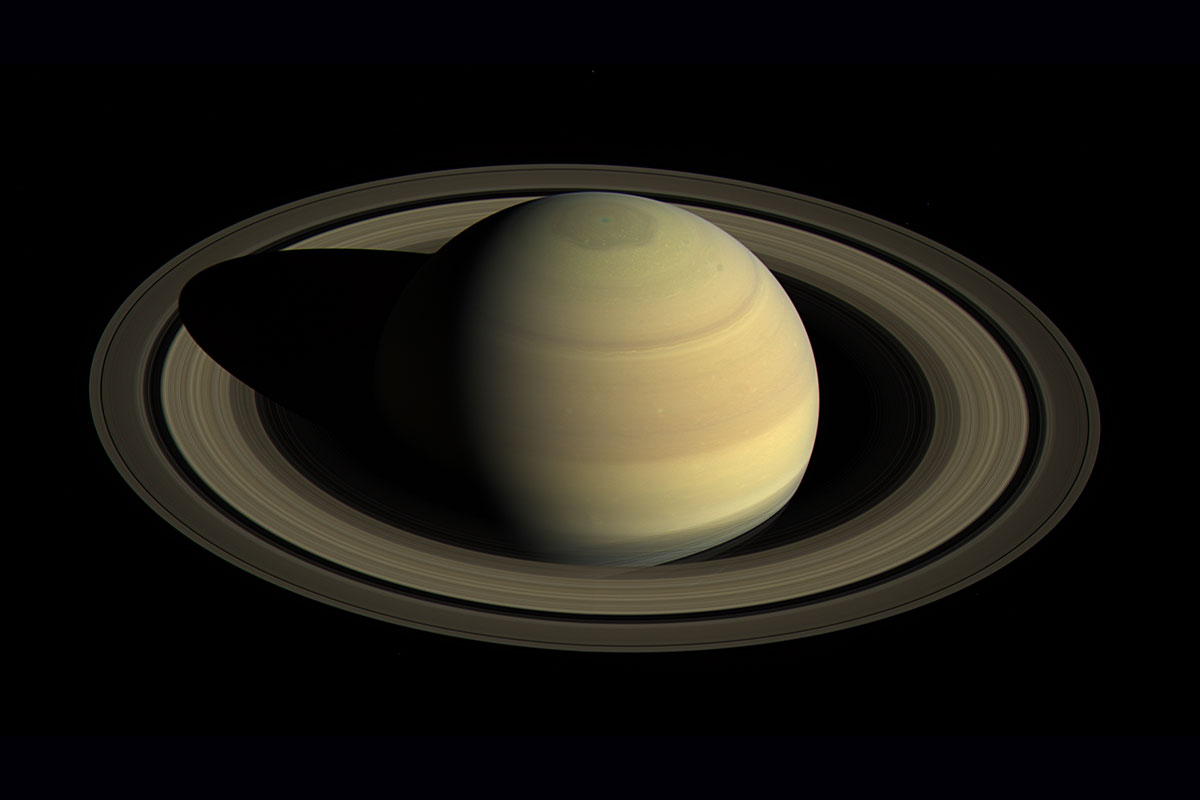
\includegraphics[width=1.56250in,height=1.04167in]{https://bakerjd99.files.wordpress.com/2017/09/cassini-saturn.jpg?w=150}

 \captionsetup[floatingfigure]{labelformat=empty}
 \begin{floatingfigure}[l]{0.25\textwidth}
 \centering
 \href{https://bakerjd99.files.wordpress.com/2017/09/cassini-saturn.jpg}{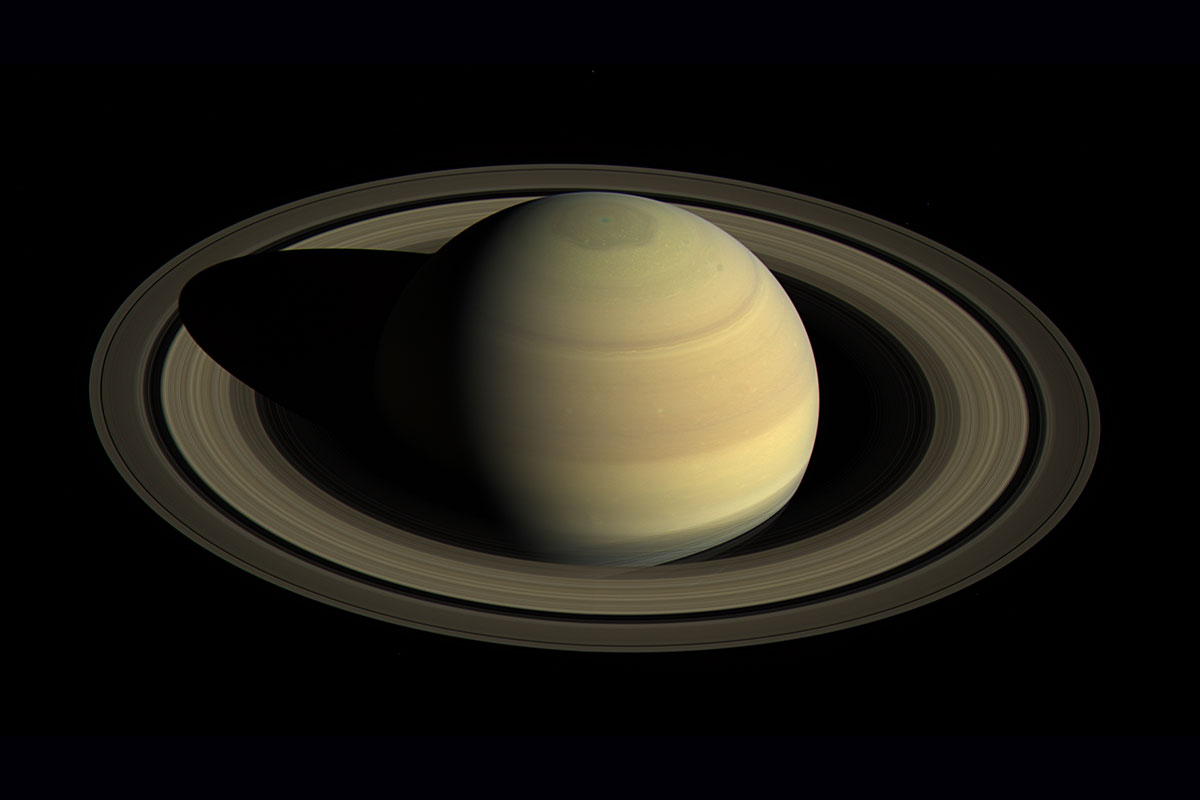
\includegraphics[width=0.235\textwidth]{cassini-saturn.jpg}}
 %\caption{}
 \label{fig:5466x0}
 \end{floatingfigure} Future
generations will remember Bill Clinton for two things, not having sex
with that woman and authorizing the launch of Cassini. I was working in
Dallas Texas in the months before Cassini's launch. It was 1997 and the
Internet was just beginning to disrupt everyday life. Google was
morphing from a thesis to a company and abominations like Facebook,
Twitter and smartphones were years away. It was a time of CD-ROM games,
56K dial-up modems, bulletin boards, hand crafted HTML websites, and
Netscape Navigator. Even in its primitive state the Internet already
exhibited many of the things I value and detest about it today. Two events
made this abundantly clear. The inane shenanigans that preceded
Cassini's launch and the death of Carl Sagan.

I had a few beefs with Sagan. Like all science popularizers he often
dumbed things down to misleading levels and, like most \emph{western}
academics, he was naive about vicious authoritarian regimes. In Sagan's
mind, a handful of exemplary Soviet scientists went a long way toward
excusing the Gulag and purges. I overlooked his good-natured naivety. It
was, and still is, a common delusion. Many intelligent people fall
victim to the belief that their superior accomplishments endow them with
universal wisdom. This is pure classic hubris.

Sagan had flaws but he was also the real scientific deal. He predicted
the surface temperature of Venus before it was measured and contributed
both scientifically and politically to the success of some of the
20\textsuperscript{th} century's most spectacular space missions like
the Martian Viking landers and the epic Voyagers. Even his popular
stunts like the
\href{https://www.space.com/17651-pioneer-10.html}{Pioneer plaque} and
the \href{https://voyager.jpl.nasa.gov/golden-record/}{Voyager gold
records} were classy and compelling. For me, Sagan's most enduring
quality was his very public and relentless refusal to buy into
irrational bullshit. He rhetorically dismembered idiots that saw faces
on Mars and skies full of alien bearing UFOs. The Martian face turned
out to an
\href{https://science.nasa.gov/science-news/science-at-nasa/2001/ast24may_1/}{eroded
mesa}, just like Sagan said it was, and we are still waiting for genuine
rigorously authenticated evidence of real UFOs. Sagan's often said,
``Extraordinary claims require extraordinary evidence!''~ It's a maxim I
apply every single day and you should too.

The day Sagan died I connected to the Internet with my trusty 56K
dial-up modem. I was looking for unofficial Sagan obituaries and boy did
I find them. It turns out that UFO cultists did not appreciate Sagan's
precise and correct analysis of their unsubstantiated nonsense. Clearly,
he was part of the vast centuries old global cover-up. Everyone knows
that the Illuminati, the Masons, the Rothschilds, the Jews, and the
Jewish aliens in the UFOs, are suppressing UFO evidence: presumably to
facilitate draining our precious bodily fluids. \emph{I exaggerate but
not by much!} It was my first encounter with unhinged Internet trolls.
My already low opinion of the people's intelligence dipped lower. Of
course, trolls come in all flavors. There are good trolls, the ones I
agree with, and evil trolls, the ones I disagree with. Overall, a free
Internet with hate mongering vicious trolls is vastly better than a
censored Internet that's been reduced to a giant empty echoing,
ruling-class-approved, safe space. ``Sticks and stones will break my
bones but words will never hurt me.''

No matter what you think of the boorish behavior of UFO cultists
celebrating Sagan's death it's clear to all, including the UFO cultists
themselves that they are, in Douglass Adam's exquisite words, ``mostly
harmless.''~ No one gives a crap what ufologists (yeah it's a word)
think and nobody will pay attention to their ravings until they meet
well-defined standards of proof. Sorry guys it's a skeptic's world and
we won't be lowering standards of scientific validation for you.

Unfortunately, anti-nuclear don't launch Cassini, nitwits almost aborted
what turned out to be an undisputed marvel of our age. I remember these
1997 loons and until they crawl out from their troglodyte caves,
prostrate themselves before the great and powerful Internet, and
publicly admit that they were completely wrong about Cassini, that
launching the probe was the right thing to do, and that some tiny risks
are very much worth taking, I will forever curse, mock, belittle, and
remind others of their appalling judgment and sniveling cowardice.

The Cassini launch hysterics began when a pack of dolts noticed the word
``Plutonium'' in Cassini's press material. Plutonium, oh my god! What
are those privileged white devils in JPL up to? The JPL white devils
tried to explain how
\href{https://saturn.jpl.nasa.gov/radioisotope-thermoelectric-generator/}{RTG
generators} work and that a safe reliable compact long-lasting power
source was required for operations at Saturn where sunlight is around
0.011 Earth's intensity but math is hard. Way too hard for ideologues
triggered by visions of Plutonium saturated Challenger like explosions
spreading deadly radiation over a wide area. It was all over hyped
rubbish. As of 2017, it's not clear that RTGs have killed a single
person in over fifty years of use let alone the tens of thousands the
Cassini Cassandras were picturing. The white devils lost patience and
did a little back of the envelope calculation that assumed a major
Cassini crash that uniformly spread the probe's ``deadly Plutonium''
over the entire Earth. Given this absurd worst case scenario, how many
excessive cancer deaths could we expect?~ The calculation
\href{https://en.wikipedia.org/wiki/Cassini\%E2\%80\%93Huygens}{estimated
about 5,000} spread over a lifetime: \emph{not enough to worry about!}
Michio Kaku called bullshit on this absurd scenario and quickly
concocted his own absurd scenario that had Cassini crashing into a dense
urban area with laser guided bomb casualty maximizing effectiveness.
This bumped the dark wet dream body count to 200,000. Both calculations
were ridiculous. This entire episode is neatly summarized in this
\href{http://www.motherjones.com/politics/1997/09/cassini-controversy/}{Mother
Jones} (can you believe it) article.

The launch of Cassini and its Earth flyby imposed miniscule risks. Even
if things went horribly, \emph{but realistically wrong}, it's unlikely
the probe would have killed more than a thousand people. Whenever I hear
projected death tolls I convert the statistic into one I care about.
\emph{What are my chances of dying?} The Earth's population was roughly
six billion in 1997. The chances of Cassini killing me was at most one
in million and probably much less. What type of whiny cowardly snowflake
would give up the glories of Cassini for one in million odds of
something bad happening? I would have accepted much worse odds.

I wasn't the only one willing to take an infinitesimal risk to advance
human knowledge. Just before Cassini's launch the anti-Cassini mob
planned a march in Washington to screech, wave banners, and go full
incontinent leftist ape. In their bush baby brains Cassini had to be
stopped. Before 1997 protesters rarely faced counter protesters but
Cassini touched a deep nerdy nerve and
\href{http://www.animatedsoftware.com/cassini/nltrs/nltr0050.htm}{a
small band of} pro-Cassini protesters showed up shouting ``Don't be a
weenie, launch Cassini,'' and like the Greeks at Marathon, they drove
the stunted grunting anti-Cassini beasts from the rhetorical field. ~I
like to imagine the ``don't be a weenie, launch Cassini'' ruckus stirred
Bill to take a break from dipping cigars in intern vaginas and get on
the phone to authorize Cassini's launch.

Today the pro-Cassini protesters would be erroneously described as
``alt-right.'' \emph{Actually, they were simply and absolutely right} as
hundreds of thousands of stunning Cassini images, thousands of
scientific papers, and dozens of unexpected discoveries about Saturn and
its Moons attest. Cassini exceeded everybody's expectations. The
Voyagers were the greatest space probes of the 20\textsuperscript{th}
century and Cassini is the greatest of the 21\textsuperscript{st} so
far. If we're lucky we'll see Cassini surpassed and that is something
to look forward to.



%\end{document}
 

